\textbf{Placing products into original floor plan layout}
\newline
\par Since the factors affecting the damage for this fixed floor plan is placing the products. The popularity of the product indicates the competitive indicates the damage. Since for each store, the number of people passing it is not equal. The store that's placed nearer to the front (cashier-entrance-exit zone) have more probability to be passed by bigger number of people. We need to place the products with high popularity on the low traffic place, the further one to the back. We can place the department which can be seen in figure 4 
\newline

\begin{center}
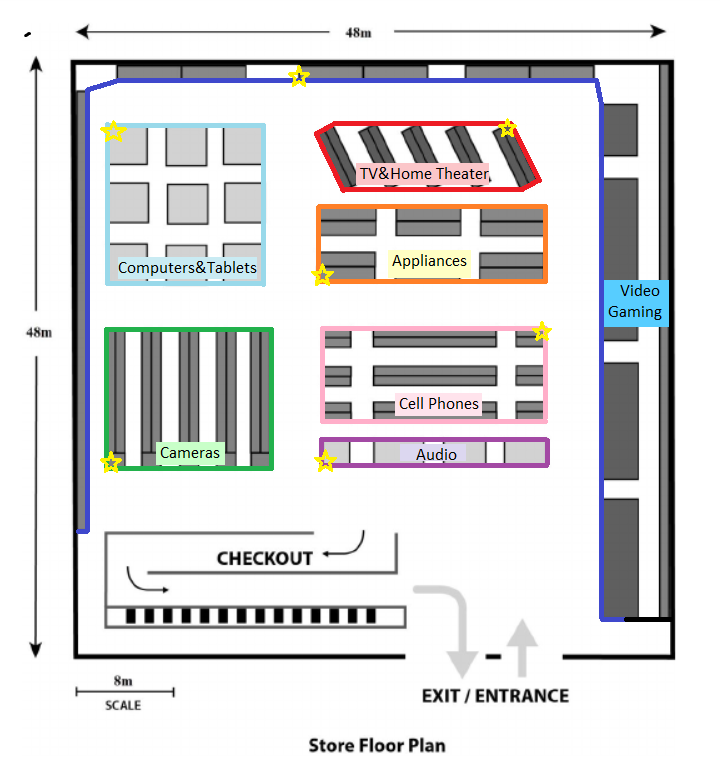
\includegraphics[width=0.6\textwidth]{fig4.4.PNG} 
\end{center}
\begin{center}
Figure 4.
\end{center}

\par The above figure represents about the strategy of ordering departments in the original floor plan layout. The plan consists of seven departments and seven stars representing the highest rating product of the department including Sport Wireless Earbud Headphones in Audio department, 5.1cu ft Freestanding Gas Range, Stainless Steel from Appliances department, Mirrorless Camera with Lens from Cameras department, Wireless Wearable Speaker - Black from Cell Phones department, 2-in-1 14" Touch-Screen Chromebook, Intel Core i3, 4GB RAM, 128GB from Computers\&Tablets department, 55" 4K UHD HDR Smart OLED TV, A8G Series from TV\&Home Theater department, and lastly, 32GB Console - Gray Joy-Con + 2 more items from Video Gaming department. Among all of the products, we found that the most popular one is the Mirrorless Cameras with Lens. Our strategy is to place the higher rating products further from the cashier-entrance-exit zone to prevent the chaos from people grabbing the valuable products. Moreover, the highest rating products of each department need to be placed far from each other enough so that they won't cause chaos, but not too far so that people can still walk around to see another products to increase the sales. \newline
\noindent \textbf{Creating new floor plan layout}
\newline
\par Since the factors that we consider having affect on the damage caused by the shoppers, for the layout one of them is the corner. We will try to build the layout with least corner possibly none. Our model will try to make them walk through a straight pathway so that there's no corner. Then we can see that having all of them walking in one pathway might not be the best way. Distributing them into many pathway might help. But if we need to distribute them into more than one pathway and then have a hole for them to pass through to get to another path, this would cause chaos and collision too. Our idea is to have them all walking in one straight way each pathway independently.
\newline
\begin{center}
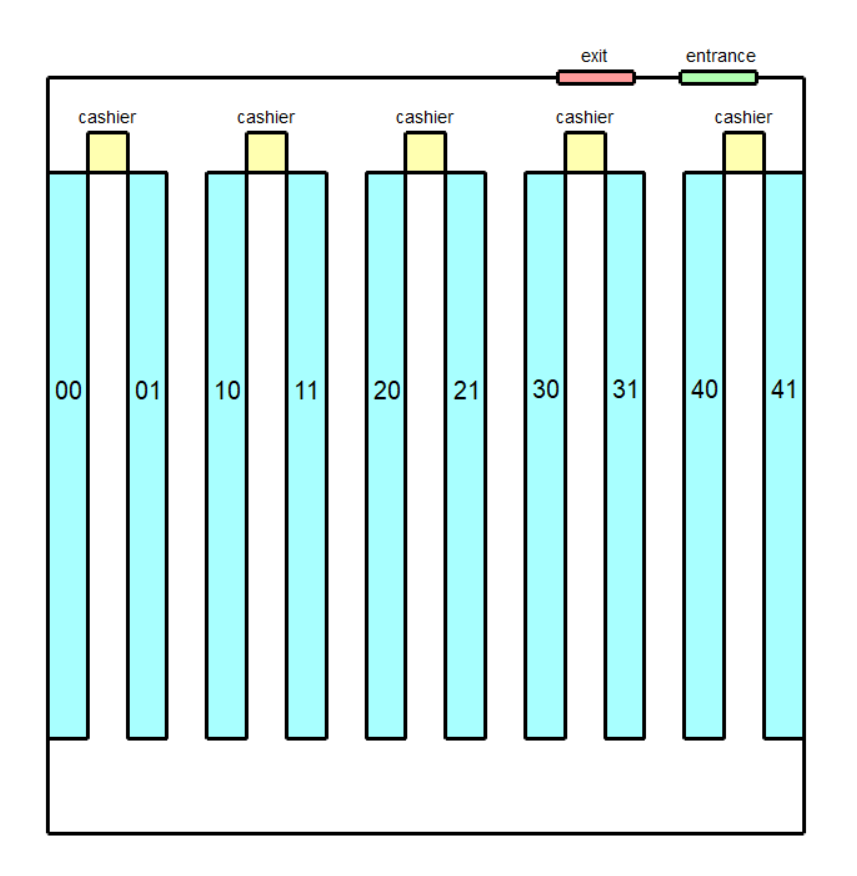
\includegraphics[width=0.6\textwidth]{fig4.1.PNG} 
\end{center}
\begin{center}
Figure 5.
\end{center}

\par From the layout, we can see that the customer will walk in through the entrance (green block in fig.4) then they would be forced to separate and enter each of the space between the shelf. The products can be accessed only from the cashier side, meaning that when the customers arrive, they will need to walk in pass the cashier through the space between each shelf, then make a u-turn to go the space that have the cashier at their ends. This layout has no corner with products, meaning reduced collision. Having them walking straight would reduce the orderlessness that occur in the original layout. After they finish picking up products they will need to pay at the cashier and then walk out at the exit. Even though the area behind that the cashier that's connected to both the entrance and the exit, the chaos would be really bad, but since there's no products to be damaged there, no damaged would be caused.
\newline

\par Then we need to place the products into the shelf. We would define each of the two shelves that can be accessed from the same space as a block. A block would contain a walkway having a cashier at its end, two shelves on the left and the right. 
\newline

\par We then need to make as much block as possible to distribute the people to minimize the chaos. Since each block is independent to the others meaning that people can't go from one block to another so each block would need to contain all the products that the customer would need. Since the products having least amount has the amount of five. We can make five blocks. (can be seen in fig.4) We expected that the alignment of the product store, and the chaos of each shopping lane to be comparable since it will equally distribute people into every lane and lower the overall chaos of the shopping hall.
\newline

\begin{center}
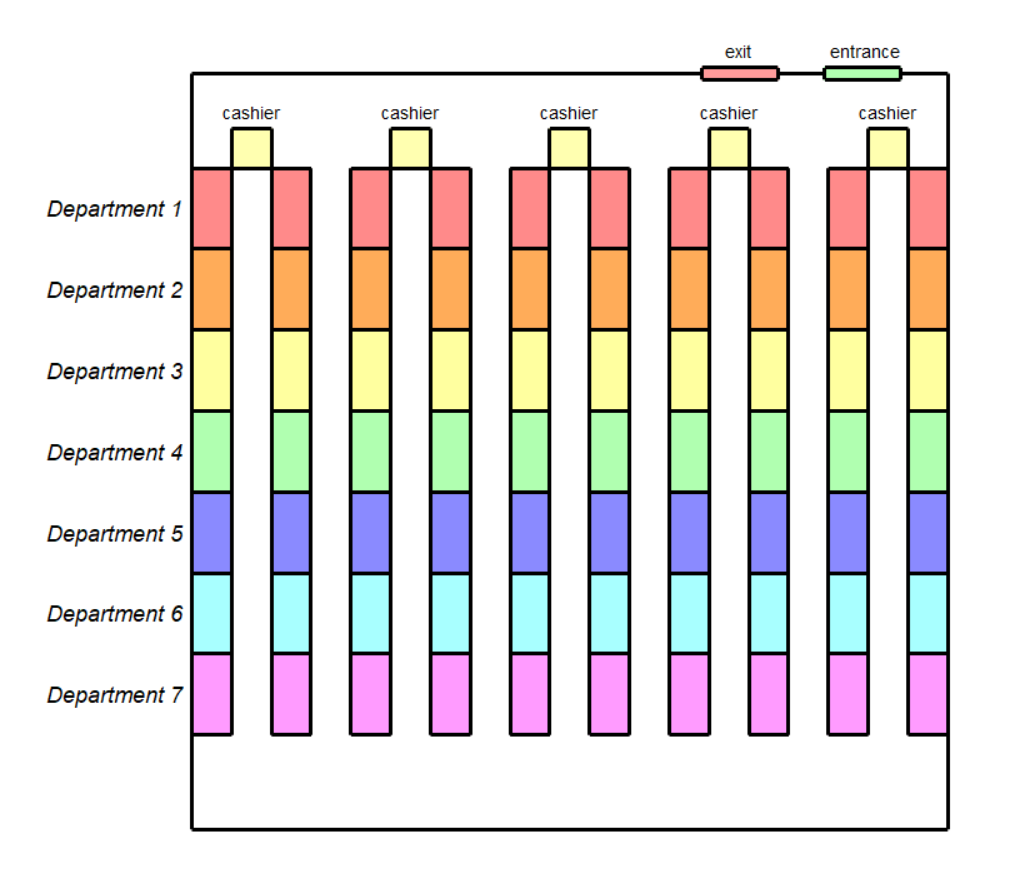
\includegraphics[width=0.7\textwidth]{fig4.2.PNG} 
\end{center}
\begin{center}
Figure 6.
\end{center}

\par Then we need to find a way to place the products. Since the products from the same department need to be placed together. We would permute the department and choose the best permutation of the department. For each permutation, we would add the products according to the permutation. (please see fig.5 for better understanding). For each department we would try to switch the products in the way that for each side of the block shelf, the messiness of the sequence of the products would be small then big then small continuously, because our model consider the messiness point as the product of its own messiness and the adjacent ones. 
\newline

\par Since calculating all the permutation by hand would be such an enormous thing to do within limited time. We would solve the problem by writing a computer program to permute and then calculate the total damage (messiness) of all the permutation and then pick the best one with minimal damage calculated based on the layout and the mathematical model.
\newline

\par Then our code will generate the products list that needed to be placed in each block separately. Then the store manager can place the products according to it to minimize the damage.
\newline

\par From our code we get that the permutation that give the optimal solution with the minimum damage is the layout below

\begin{center}
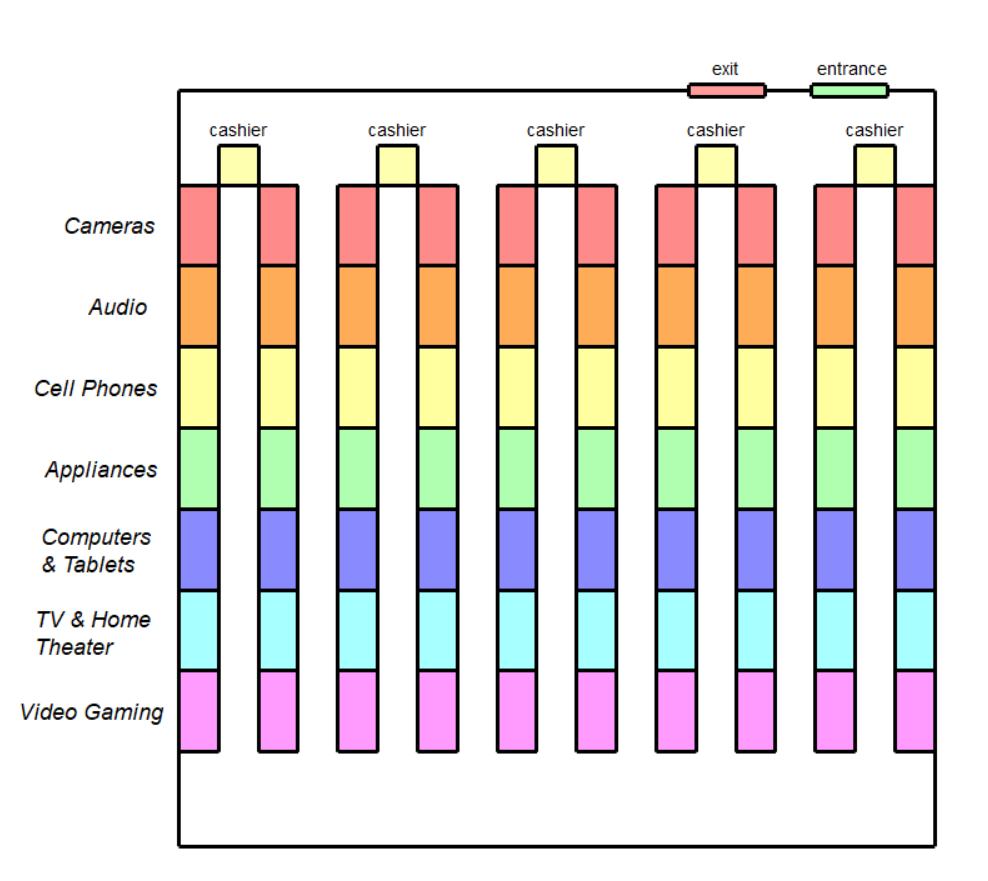
\includegraphics[width=0.7\textwidth]{fig4.3.PNG} 
\end{center}
\begin{center}
Figure 7.
\end{center}
